\section{Wall distance computation methods}
\label{sec:walldist}
Calculation of the wall distance $d$ is required in order to solve the Spalart-Allmaras equation. In the literature, it is typically computed in one of two ways:
\begin{enumerate}
    \item by a brute force approach.
    \item by solving an additional PDE.
\end{enumerate}
The brute force approach is straight-forward and consists of looping through every CV and finding the nearest wall, which itself is done by looping over every face lying on the solid boundary. Depending on the mesh, this approach can be very costly~\cite{tucker2005computations}. Moreover, some codes approximate the wall distance for a field point $P$ as the distance between $P$ and the nearest node or face center lying on a solid boundary, as opposed to calculating the perpendicular distance between a point and a plane, which is more costly. This approximation and the potential error are illustrated in~\Cref{fig:nasawalldist}.
\begin{figure}
    \centering
    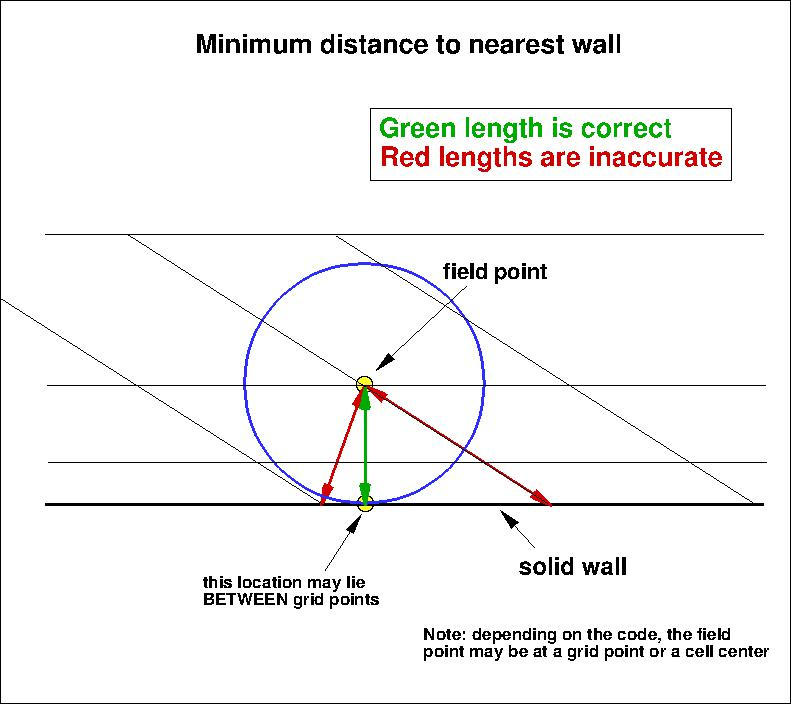
\includegraphics[width=0.55\textwidth]{figs/mindist}
    \caption{Common approximation made in brute force wall distance calculations~\cite{tmr}.}
    \label{fig:nasawalldist}
\end{figure}

The other approach, solving an additional PDE, may seem like a lot of extra work. However, CFD codes already provide functions and data structures required in solving such equations. There exists many different equations for approximating the wall distance, which are detailed and compared in~\cite{tucker2005computations,tucker2011hybrid,belyaev2015variational}. The technique used in syn3D and NX Flow consists in solving a Poisson equation followed by a normalization, which can mathematically be written as:
\begin{align}
    \begin{split}
    \nabla^2\phi &= -1\\
    d &= ||\nabla\phi||_2 + \sqrt{
        ||\nabla\phi||_2 + 2\phi
    }
    \end{split}
    \label{eq:poissondist}.
\end{align}
A homogeneous Dirichlet BC is to be imposed on $\phi$ at solid walls and a homogeneous Neumann BC at all other boundaries. The approximation of $d$ by~\Cref{eq:poissondist} is only accurate close to walls, however that is the only location where an accurate $d$ is needed when it comes to turbulence modelling.